\chapter{galvoChar}
\newcommand \galvo {Galvanometer-Spiegel}
\newcommand \bildwidth {0.95\textwidth}

% bild{h!}{}{}{}
% #1 float position
% #2 filename.ext
% #3 cap
% #4 label
\newcommand \bild[4]{\begin{figure}[#1]	\centering	\includegraphics[width=\bildwidth]{pics/#2}	\caption{#3}	\label{#4}	\end{figure}}


% \begin{abstract}
OCT-Systeme (optical coherence tomography) ermitteln punktweise, tiefenaufgeloeste Geometrie-Daten in transparenten Materialien. Zur Ermittlung von 3-dimensionalen Datensaetzen wird der Messpunkt dabei mit \galvo n im X/Y-Betrieb verfahren. Dies sind hochdynamische Drehantriebe fuer optische Anwendungen, die mit einer Rate von etwa 500Hz vor- und rueckwaerts rotieren koennen. Sie tragen mitrotierende Spiegel, um den optischen Pfad auszulenken und somit flaechige Scans zu ermoeglichen. \\ 
Handelsuebliche Galvanometer-Spiegel besitzen mechanische Traegheiten, die bei Scan-Raten ab 800Hz keine maximale Auslenkung mehr erlauben. Dadurch wird bei hohen Geschwindigkeiten der optische Messbereich eingeschraenkt. An realen, vorhandenen \galvo wird durch Messungen diese Traegheit charakterisiert und modelliert. Dieses Modell soll als Basis dienen, um adaptierte Steuersignale zu erzeugen, die die angesprochenen Traegheiten Ausgleichen.\\
% \end{abstract}

% \begin{IEEEkeywords}
OCT-System, Galvanometer-Scanner, Regelungstechnik, Laser-Scanner, Interferometrie, dynamische Modellierung
% \end{IEEEkeywords}

% \section{Einleitung}
	% \subsection{Optische Kohaerenz-Tomographie}
% Optische Kohaerenz Tomographie (optical coherence tomography, OCT) ist ein bildgebendes Messverfahren zur Analyse von transparenten und opaken Materialien und weist aehnlichkeiten zu den Messprozessen via Ultraschall oder Radar auf. Die Probe, die vermessen werden soll, wird mit einer elektromagnetischen Welle beaufschlagt, die resultierenden 'Echos' werden bezueglich ihrer resultierenden Laufzeiten analysiert. Aus diesen Laufzeiten wiederum ergibt sich die geometrische Struktur, die den Schichtaufbau der Probe, oder auch die maximale Eindringtiefe der Welle enthaelt. So entsteht ein tiefenaufgeloester Messpunkt. In der Regel wird diese EM-Welle aus einer kohaerenten, breitbandigen Lichtquelle im sichtbaren bis in den nahen Infrarot-Bereich erzeugt. Kohaerenz bedeutet, dass mehrere Wellenzuege einer Lichtquelle eine feste Phasenbeziehung zueinander haben muessen. Dies ist notwendig, um stabile Interferenzmuster zu erhalten. Zur Detektion der Echos reichen jedoch keine herkoemmlichen Opto-Detektoren oder Kameras aus, einerseits aufgrund der Ausbreitungsgeschwindigkeit des Lichtes, andererseits an den geringen reflektierten Lichtintensitaeten. Deshalb kommt Interferometrie zum Einsatz, um die Eindringtiefe eines Photons zu ermitteln, das von einer Probe reflektiert wird. \\ Bei Interferometrie wird der Laserstrahl gesplittet und eine Welle auf einen optischen Referenzenpfad bekannter Laenge gesendet, die andere auf die Oberflaeche des Prueflings. Die Reflexionen, also die ruecklaufenden Wellen werden ueberlagert und erzeugen je nach Beschaffenheit des Probenmaterials konstruktive oder destruktive Interferenz. Diese Interferenz kann mittels eines Opto-Detektors\footnote{time-domain OCT, swept-source},  oder eines Spektrometers\footnote{ spectral domain - OCT }  gesampelt und weiterverarbeitet werden. Ein einzelner vermessener Punkt und seine Tiefeninformation ueber das betrachtete Material wird als A-Scan bezeichnet. Aggregiert man eine Menge von A-Scans entlang einer Linie (X-Richtung) ueber das Probenmaterial, bildet dies einen B-Scan und die Aggregation von B-Scans entlang einer Linie in Y-Richtung ergibt einen Volumen-Scan, also ein raeumliches, ein dreidimensionales Abbild des Probenmaterials. Relevante Parameter von OCT-Systemen sind die Eindringtiefe, der axiale und laterale Messbereich, axiale und laterale Aufloesung und die Messgeschwindigkeit. Betraegt die Eindringtiefe bei Ultraschall typischerweise einige Zentimeter und eine Aufloesung im Millimeter-Bereich, so erlaubt OCT nur wenige Millimeter unter die Oberflaeche zu schauen, jedoch mit Mikrometer-Aufloesungen. Abmessbare Bereiche bewegen sich bei Ultraschall in der Groessenordnung von Zentimetern, bei OCT in Millimetern\cite{WhitepaperEO}. Erreichbare Geschwindigkeiten ergeben sich aus A-Scan-Raten bis 100kHz. \\  
Die Bezeichnung 'optische Kohaerenz-Tomographie' ergibt sich einerseits aus der kohaerenten Lichtquelle. Andererseits stehen die Namensteile 'tomos' fuer Schnitt oder Sektion, und 'graphein' fuer Schreiben oder Zeichnen, und stammen beide aus dem Griechischen. Sie spiegeln wider, dass das entstehende Abbild aus einzelnen Sektionen oder Schnittbildern zusammengesetzt wird. Das Manipulieren des Lichtstrahls entlang der erwaehnten Linien erfolgt mit rotierbar gelagerten Spiegeln, einen fuer die X- einen fuer die Y-Richtung. Je schneller diese Rotation moeglich ist, desto schneller koennen OCT-Bilder erstellt werden. Eine weitverbreitete technische Realisierung, die sehr schnelles Rotieren der Spiegel erlaubt, heisst \galvo .
\bild{h!}{DetailGalvoOn}{Anordnung von XY-\galvo n}{DetailGalvoOn}

% \subsection{ \galvo }
% Bei \galvo n (auch: Galvos) handelt es sich um hochdynamische opto-mechanische Komponenten, die auf dem klassischen Galvanometer nach Hans Christian Oersted basieren: Ein rotierbar gelagertes, magnetisierbares Objekt, zB. eine Magnetnadel, wird in der Naehe eines stromdurchflossenen Leiters aus seiner Ruhelage ausgelenkt. Die geringe Empfindlichkeit der Auslenkung gegenueber dem Strom wird verbessert, indem eine hohe Wicklungszahl des elektr. Leiters um das auszulenkende Objekt gelegt wird und somit eine elektrische Induktivitaet, eine Spule, entsteht. Der nichtlineare Zusammenhang zwischen Strom und Auslenkwinkel kann durch Lagerung der Spule zwischen einem starr angebrachten Eisenzylinder innerhalb und einem Dauermagneten, der ausserhalb der Spule angeordnet ist, in guter Naeherung linearisiert werden\cite{keithleyHistory}. Wird dieses klassische Galvanometer mit einem Spiegel als rotierbares Objekt erweitert, lassen sich damit optische Pfade, konkret: der Strahlengang einer punktfoermigen Lichtquelle in einer Raumdimension manipulieren. Praktikabel fuer technische Anwendungen ist, dass diese Manipulation einigermassen linear per Strom oder Spannung an der Galvo-Spule gesteuert werden kann. Bei den vorliegenden \galvo n ist eine Leistungselektronik enthalten, die fuer die Umsetzung von Steuersignalen auf die erforderlichen Stroeme und Spannungen sorgt, im Folgenden wird deshalb nurmehr von Steuersignalen gesprochen. Kombiniert man zwei \galvo n in geeigneter geometrischer Anordnung und bestrahlt diese mit einem Punktlaser, so laesst sich dieser Punkt im 2-Dimensionalen manipulieren. Eine solche Anordnung ist in Abb.~\ref{DetailGalvoOn} dargestellt. Bei ausreichender Geschwindigkeit, mit der der Laser-Punkt ausgelenkt wird, koennen 2D-Konturen projiziert werden, die fuer das menschliche Auge ein 'stehendes' Bild darstellen. So werden diese Komponenten fuer Laser-Shows eingesetzt. Handelsueblich werden diese Komponenten als Laser-Scanner bezeichnet und fuer Lichteffekte bei Musikveranstaltungen, Kunst-Installationen und Diskotheken eingesetzt. Auf OCT-Systeme appliziert, koennen Galvanometer-Spiegel hingegen genutzt werden, um die optische Wirkung einer kohaerenten Lichtquelle nicht auf einen Ortspunkt beschraenkt zu nutzen, sondern auf einer gewisse Flaeche verteilt an eine beliebige Stelle einer zu untersuchenden Probe zu projizieren. Werden ein X- und ein Y-Galvo jeweils mit einer langsamen und einer schnellen Rampe angesteuert, ergibt dies ein Rechteck auf der Probe, die gewuenschte 'Bildform' des Laserpunktes fuer OCT-Systeme. So koennen Proben rasterfoermig abgescannt werden.

\subsection{Motivation}
Die beschriebenen Eigenschaften, speziell der lineare Zusammenhang, gelten, bei guenstigen handelsueblichen \galvo n aus der Showlaser-Branche, fuer langsame Auslenkungen von $\le$800Hz. Schnellere Steuersignale fuehren zwar auch zu schnelleren Rotationen und erlauben somit schneller Messungen. Jedoch folgt die innere Mechanik des Spiegels dann  nicht mehr mit dem vollen Auslenk-Winkel. Auf eine technische Anwendung umgelegt, bedeutet dies, dass dann nicht mehr die volle Flaeche abgerastert werden kann. Offensichtlich liegt dies an der Massentraegheit der rotierbaren Komponenten, vermutet wird ein Tiefpass-Verhalten zwischen Steuersignal und Auslenkwinkel. Dieser Zusammenhang wird im Folgenden experimentell untersucht, um konkrete Aussagen ueber die Traegheit und deren Konsequenzen machen zu koennen und weiters, um mit adaptierten Steuersignalen auch bei hoeheren Frequenzen ($\sim 1000 ... 3500Hz$) volle Auslenkwinkel nutzen zu koennen. Abb.~\ref{SawVsSpline} zeigt ein moegliches adaptiertes Steuersignal. Das unterstellte Tiefpass-Verhalten wuerde auch eine Phasenverschiebung zwischen Steuersignal und Winkel implizieren, die ebenfalls untersucht wird.
\bild{h!}{SawVsSpline.eps}{bestehendes und adaptiertes Steuersignal}{SawVsSpline}
% \footnote{Diskotheken, Konzerte, Kunstinstallationen}
\section{Recherche}
\subsection{dynamisches Modell}
Die Modellierung erfolgt auf Basis experimenteller Untersuchung des Zusammenhangs zwischen Steuerspannung und Auslenkwinkel mit Methoden der Regelungstechnik. Einen vergleichbaren Ansatz haben Rasoanarivo et al. \cite{SLMGalvos:Rasoanarivo} gewaehlt, um Galvanometer-Spiegel zur Anwendung beim selektiven Laserschmelzen in der additiven Fertigung zu untersuchen. Dort wurde das bewegliche System als Gleichstrommotor mit uebertragungsfunktion 2ter-Ordnung modelliert. Selbigen Ansatz legt auch die Regelungstechnik nahe: Die beweglichen Komponenten werden als rotatorisches Starrkoerper-System angesehen, das ueber elektrische Induktion angeregt wird. Eine dynamische Vermessung per Sprungantwort eruebrigt sich, da zur Detektion notwendiges Equipment, zum Beispiel eine High-Speed-Kamera, nicht zur Verfuegung steht. Stattdessen fiel die Entscheidung auf Anregung mit Sinus-Signalen schrittweise steigender Frequenz und Aufnahme der resultierenden Projektion eines so abgelenkten Laserstrahles.
\subsubsection{	kpps versus dynamisches Modell}
In der Branche der Showlaser, aus der das Testobjekt stammt, ist zur Charakterisierung die Einheit 'kpps' gebraeuchlich und steht fuer 'kilo points per second', also wievielmal tausend Bildpunkte pro Sekunde projiziert werden koennen\cite{ildaHomepage}. Genaugenommen lautet die Bezeichnung 'kpps@8gradILDA' und bezieht sich auf eine Auslenkung von 8grad und Darstellung eines Testbildes nach ILDA\footnote{International Laser Display Association, definiert Standards fuer Showlaser}. Dies mag die Tauglichkeit eines \galvo s fuer Laser-Shows ausreichend beschreiben, ist jedoch fuer die Anwendung in OCT-Systemen nicht aussagekraeftig, da Dynamik in der Form 'Punkte pro Zeiteinheit' auf den gewuenschten kontinuierlichen Betrieb nicht umlegbar ist. Insbesondere, da in dieser Kennzahl Traegheiten sowohl fuer x- als auch y-Achse vermengt sind. Ausserdem wird auch nur der lineare Bereich getestet. Da dies die einzige dynamische Kennzahl von Schowlaser-\galvo n ist, bleibt nichts anders uebrig als selbst zu messen und zu modellieren.
% \subsection{ebay vs Sino vs Camebridge}
\section{Messungen}
Beim Testobjekt handelt es sich um einen 'RGB-SCAN20, 20Kpps galvanometer scanner', der Marke 'RGB-lasers'. Die Aufnahme der Auslenkungs-Amplitude erfolgt durch Vermessen des projizierten Laserpunktes mit Massband und freiem Auge, der Phasenlage durch einen Opto-Detektor, der auf der '0'-Linie des Strahlengangs sitzt. Abb.~\ref{ImageMeasure01} zeigt das ablesbare Amplituden-Bild einer Messung. Die kohaerenten Lichtquellen, die ueblicherweise in OCT-Systemen zum Einsatz kommen, sind nicht im menschlich sichtbaren Bereich verfuegbar, weshalb stattdessen ein roter Punkt-Laser zum Einsatz kommt. Auch saemtliche Komponenten der Interferometrie und deren Detektion tragen nichts zur Analyse der Galvo-Dynamik bei und sind deshalb nicht Teil der Messungen. Abb.~\ref{DutTop02} zeigt die Aufspannung des Testobjekts links, der Laser-Lichtquelle rechts, sowie der Treiber-Elektronik, ueber die Sinus-Signale auf das Testobjekt appliziert werden.
\begin{figure}[h!]	\centering	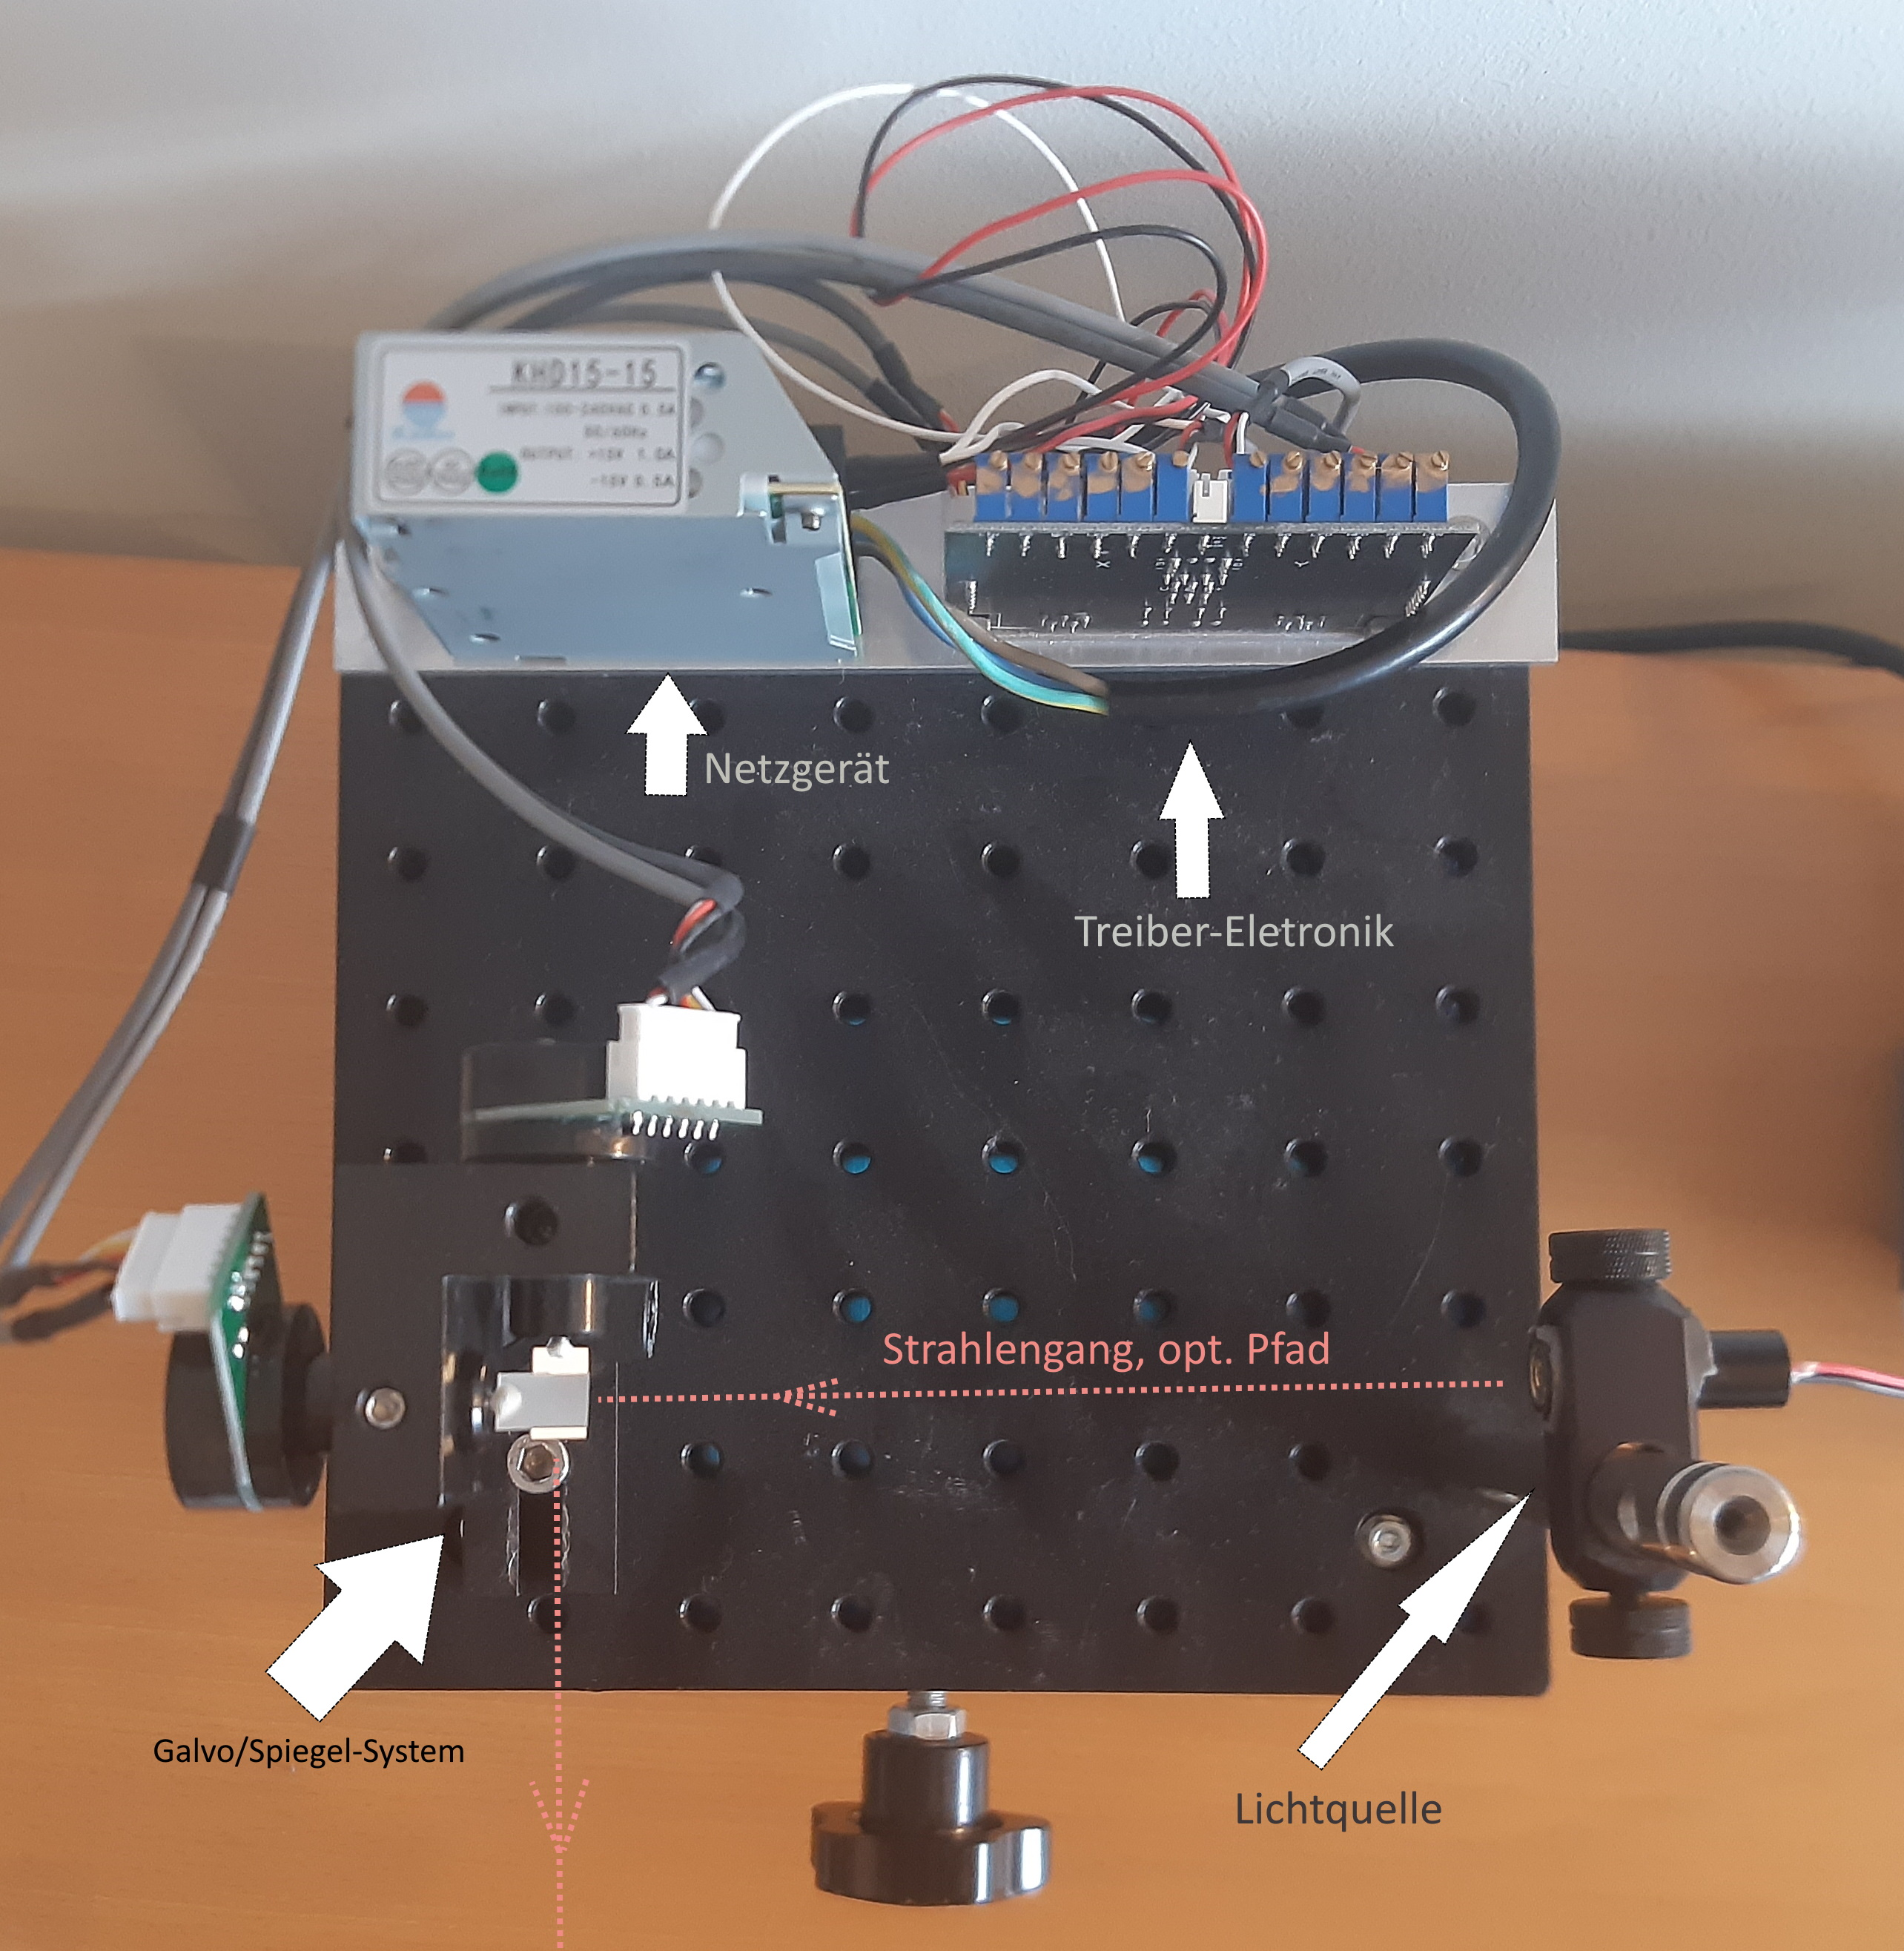
\includegraphics[width=\bildwidth]{pics/DutTop02.jpg}	\caption{Aufspannung des Testobjekts}	\label{DutTop02}	\end{figure}
\subsection{Konzept}
Um Messdaten fuer das Modell zu erhalten, werden die Galvanometer-Spiegel mit einem Laser-Strahl beleuchtet, wodurch diese in Ruheposition den Strahl rechtwinkelig umlenken und einen Laser-Punkt auf eine gegenueberliegende Flaeche projizieren. Weiters werden die Galvanometer-Spiegel separat mit sinusfoermigen Signalen angesteuert, wodurch ihre Spiegel rotiert werden. Dadurch wird der Punkt in x-, respektive, y-Richtung ausgelenkt. Bei langsamer Auslenkung mit einem Sinus von $\sim$1Hz bleibt die Projektion fuer das menschliche Auge noch deutlich als Punkt erkennbar, ab 5Hz entsteht der Eindruck einer ruckelnden Linie und bei 40Hz eine deutlich sichtbare Linie ohne erkennbares Zittern. Die Geometrie aus Messaufbau und Projektionsflaeche wird konstant gehalten und die Hoehe dieser Linie als Auslenkung herangezogen. Weiters wird im Punkt des Nulldurchgangs ein Opto-Detektor platziert, mit dem die Phasenlage des Laser-Strahl zum Steuersignal in Bezug gesetzt wird, dargestellt in Abb.~\ref{DetektorsForPhase}. Da das verwendete Massband eine spuerbare Flexibilitaet aufweist, wurde es auf Masshaltigkeit ueberprueft. Per Schieblehre nachgemessen, hat es nach dem Aufkleben auf eine Projektionsflaeche eine Abweichung $\le$ 1mm. Der Normalabstand zwischen Messobjekt und Projektionsflaeche betraegt 3200mm.
% \subsection{Aufbau}
	% \begin{equation}
	% d = 3190mm
	% \end{equation}
% \begin{figure}[h!]	\centering	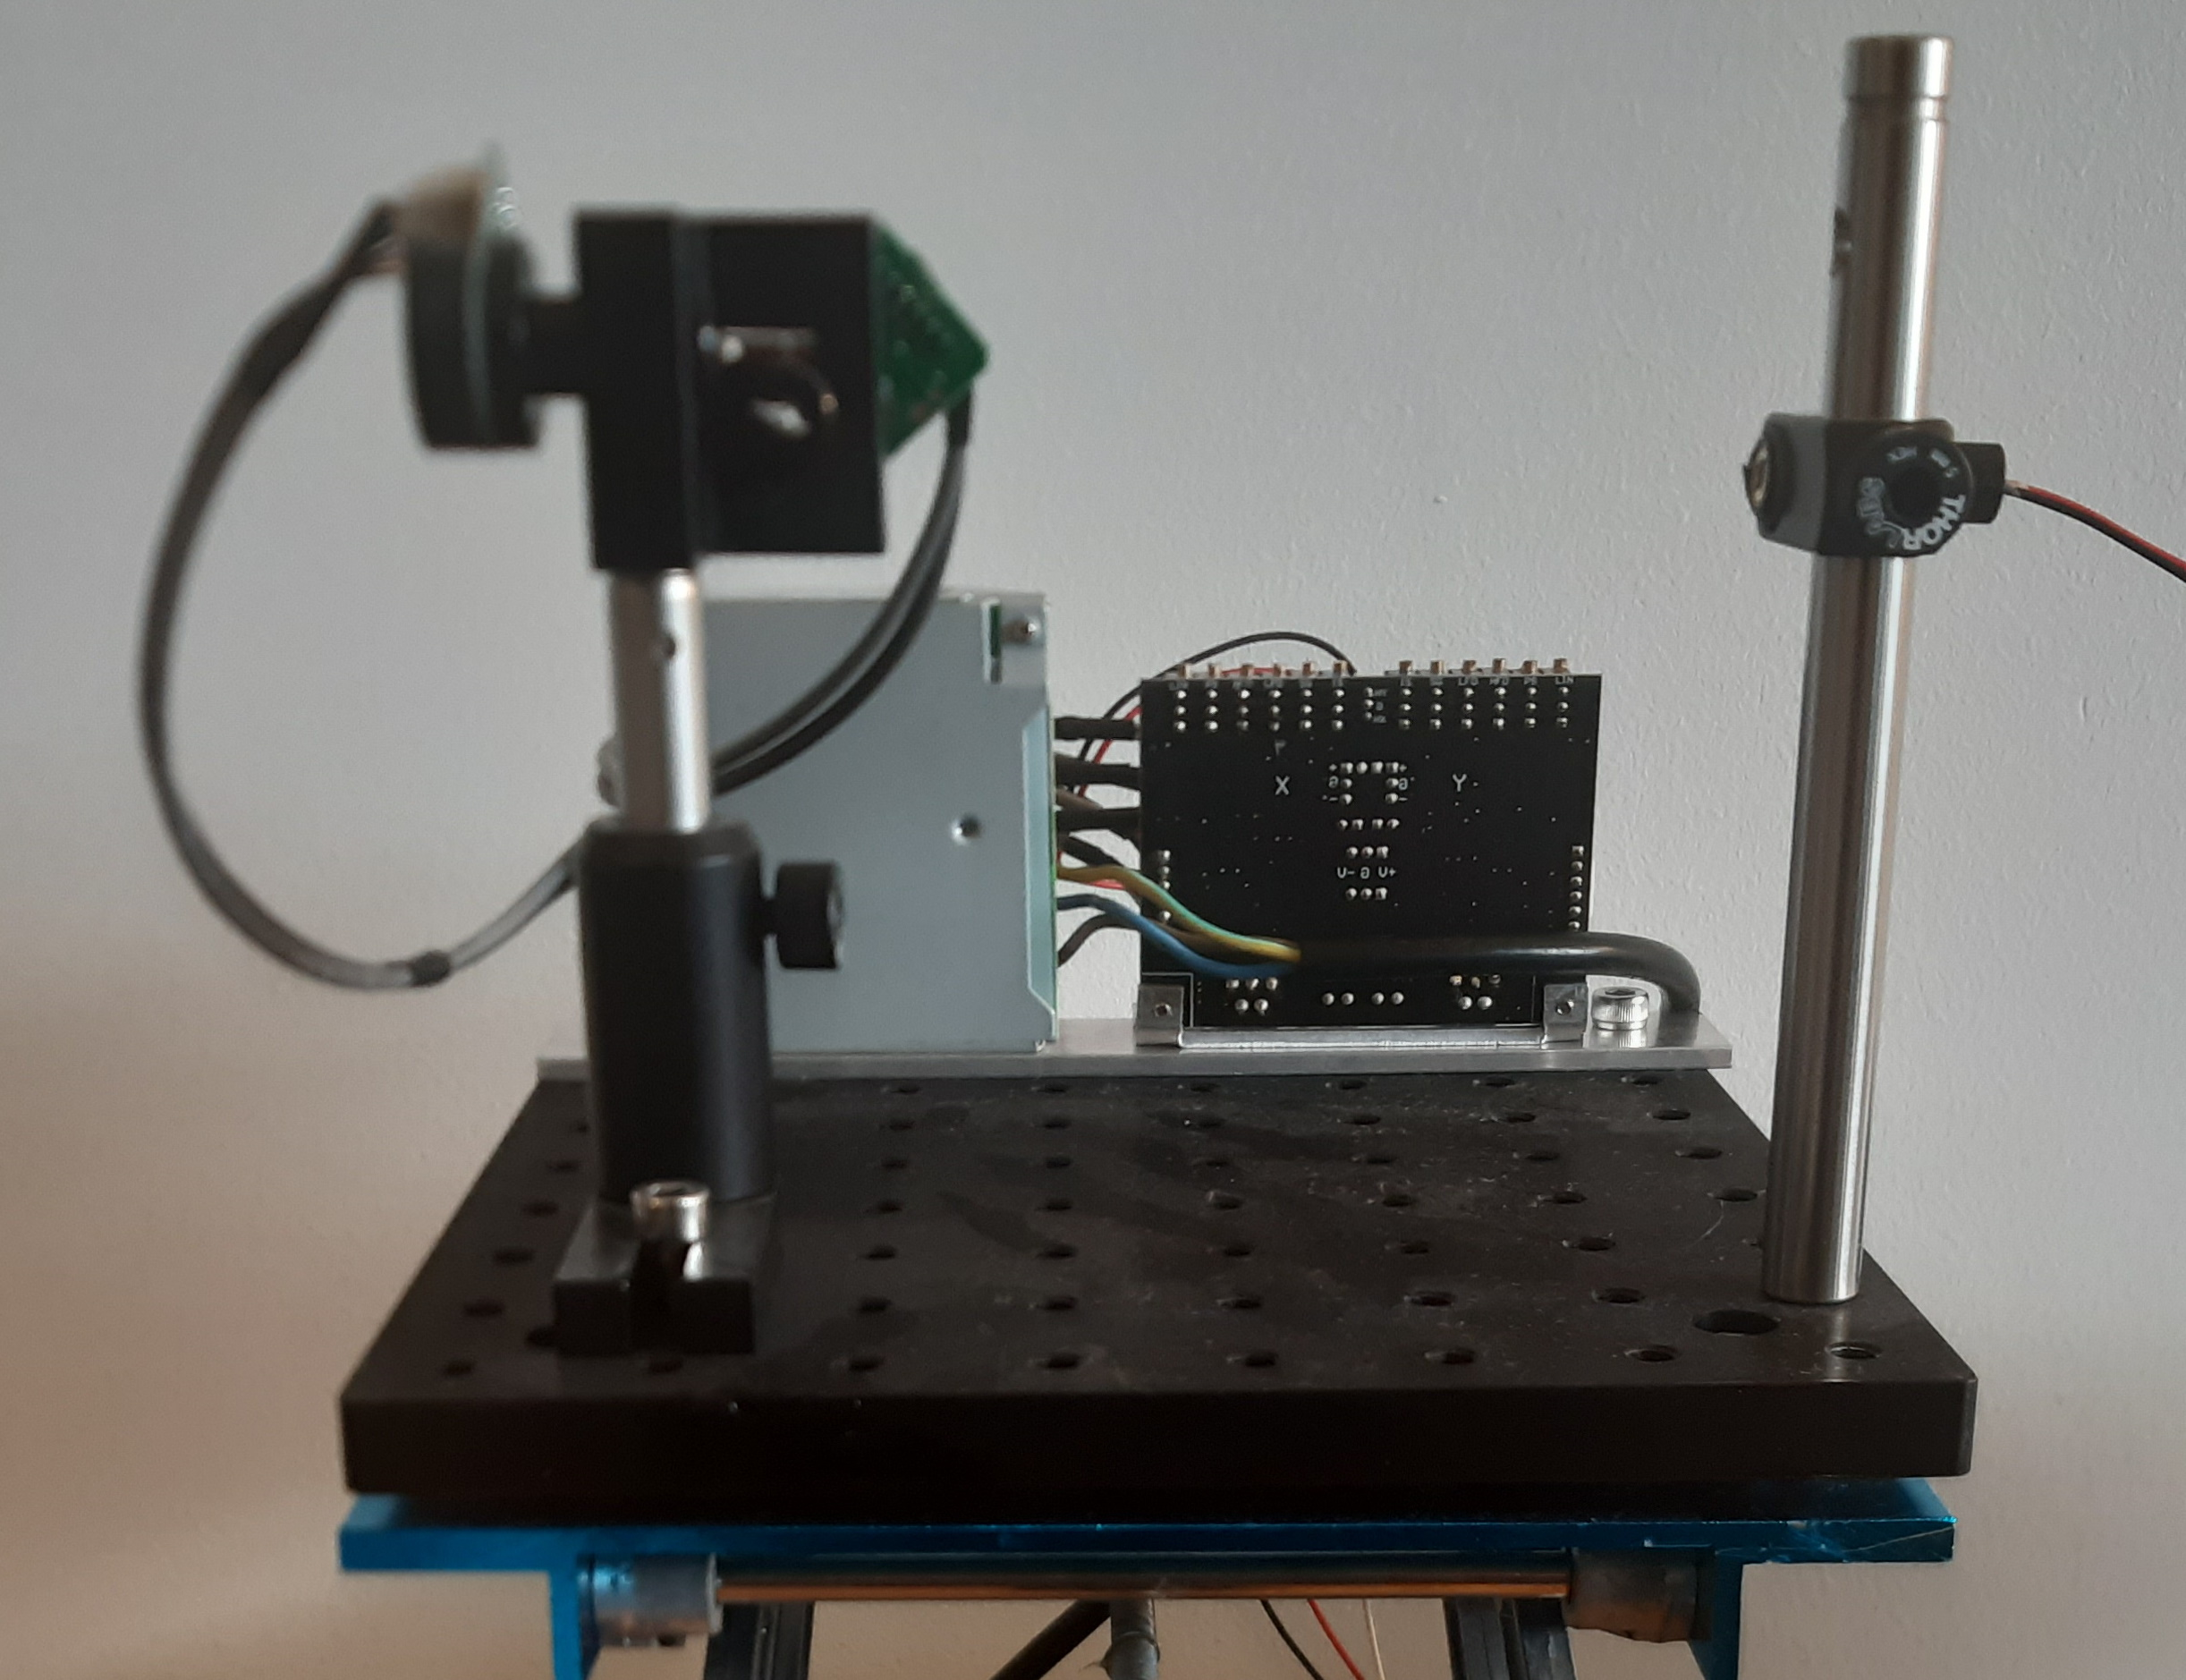
\includegraphics[width=\bildwidth]{pics/DutFront01.jpg}	\caption{DutFront01}	\label{DutFront01}	\end{figure}
% \begin{figure}[h!]	\centering	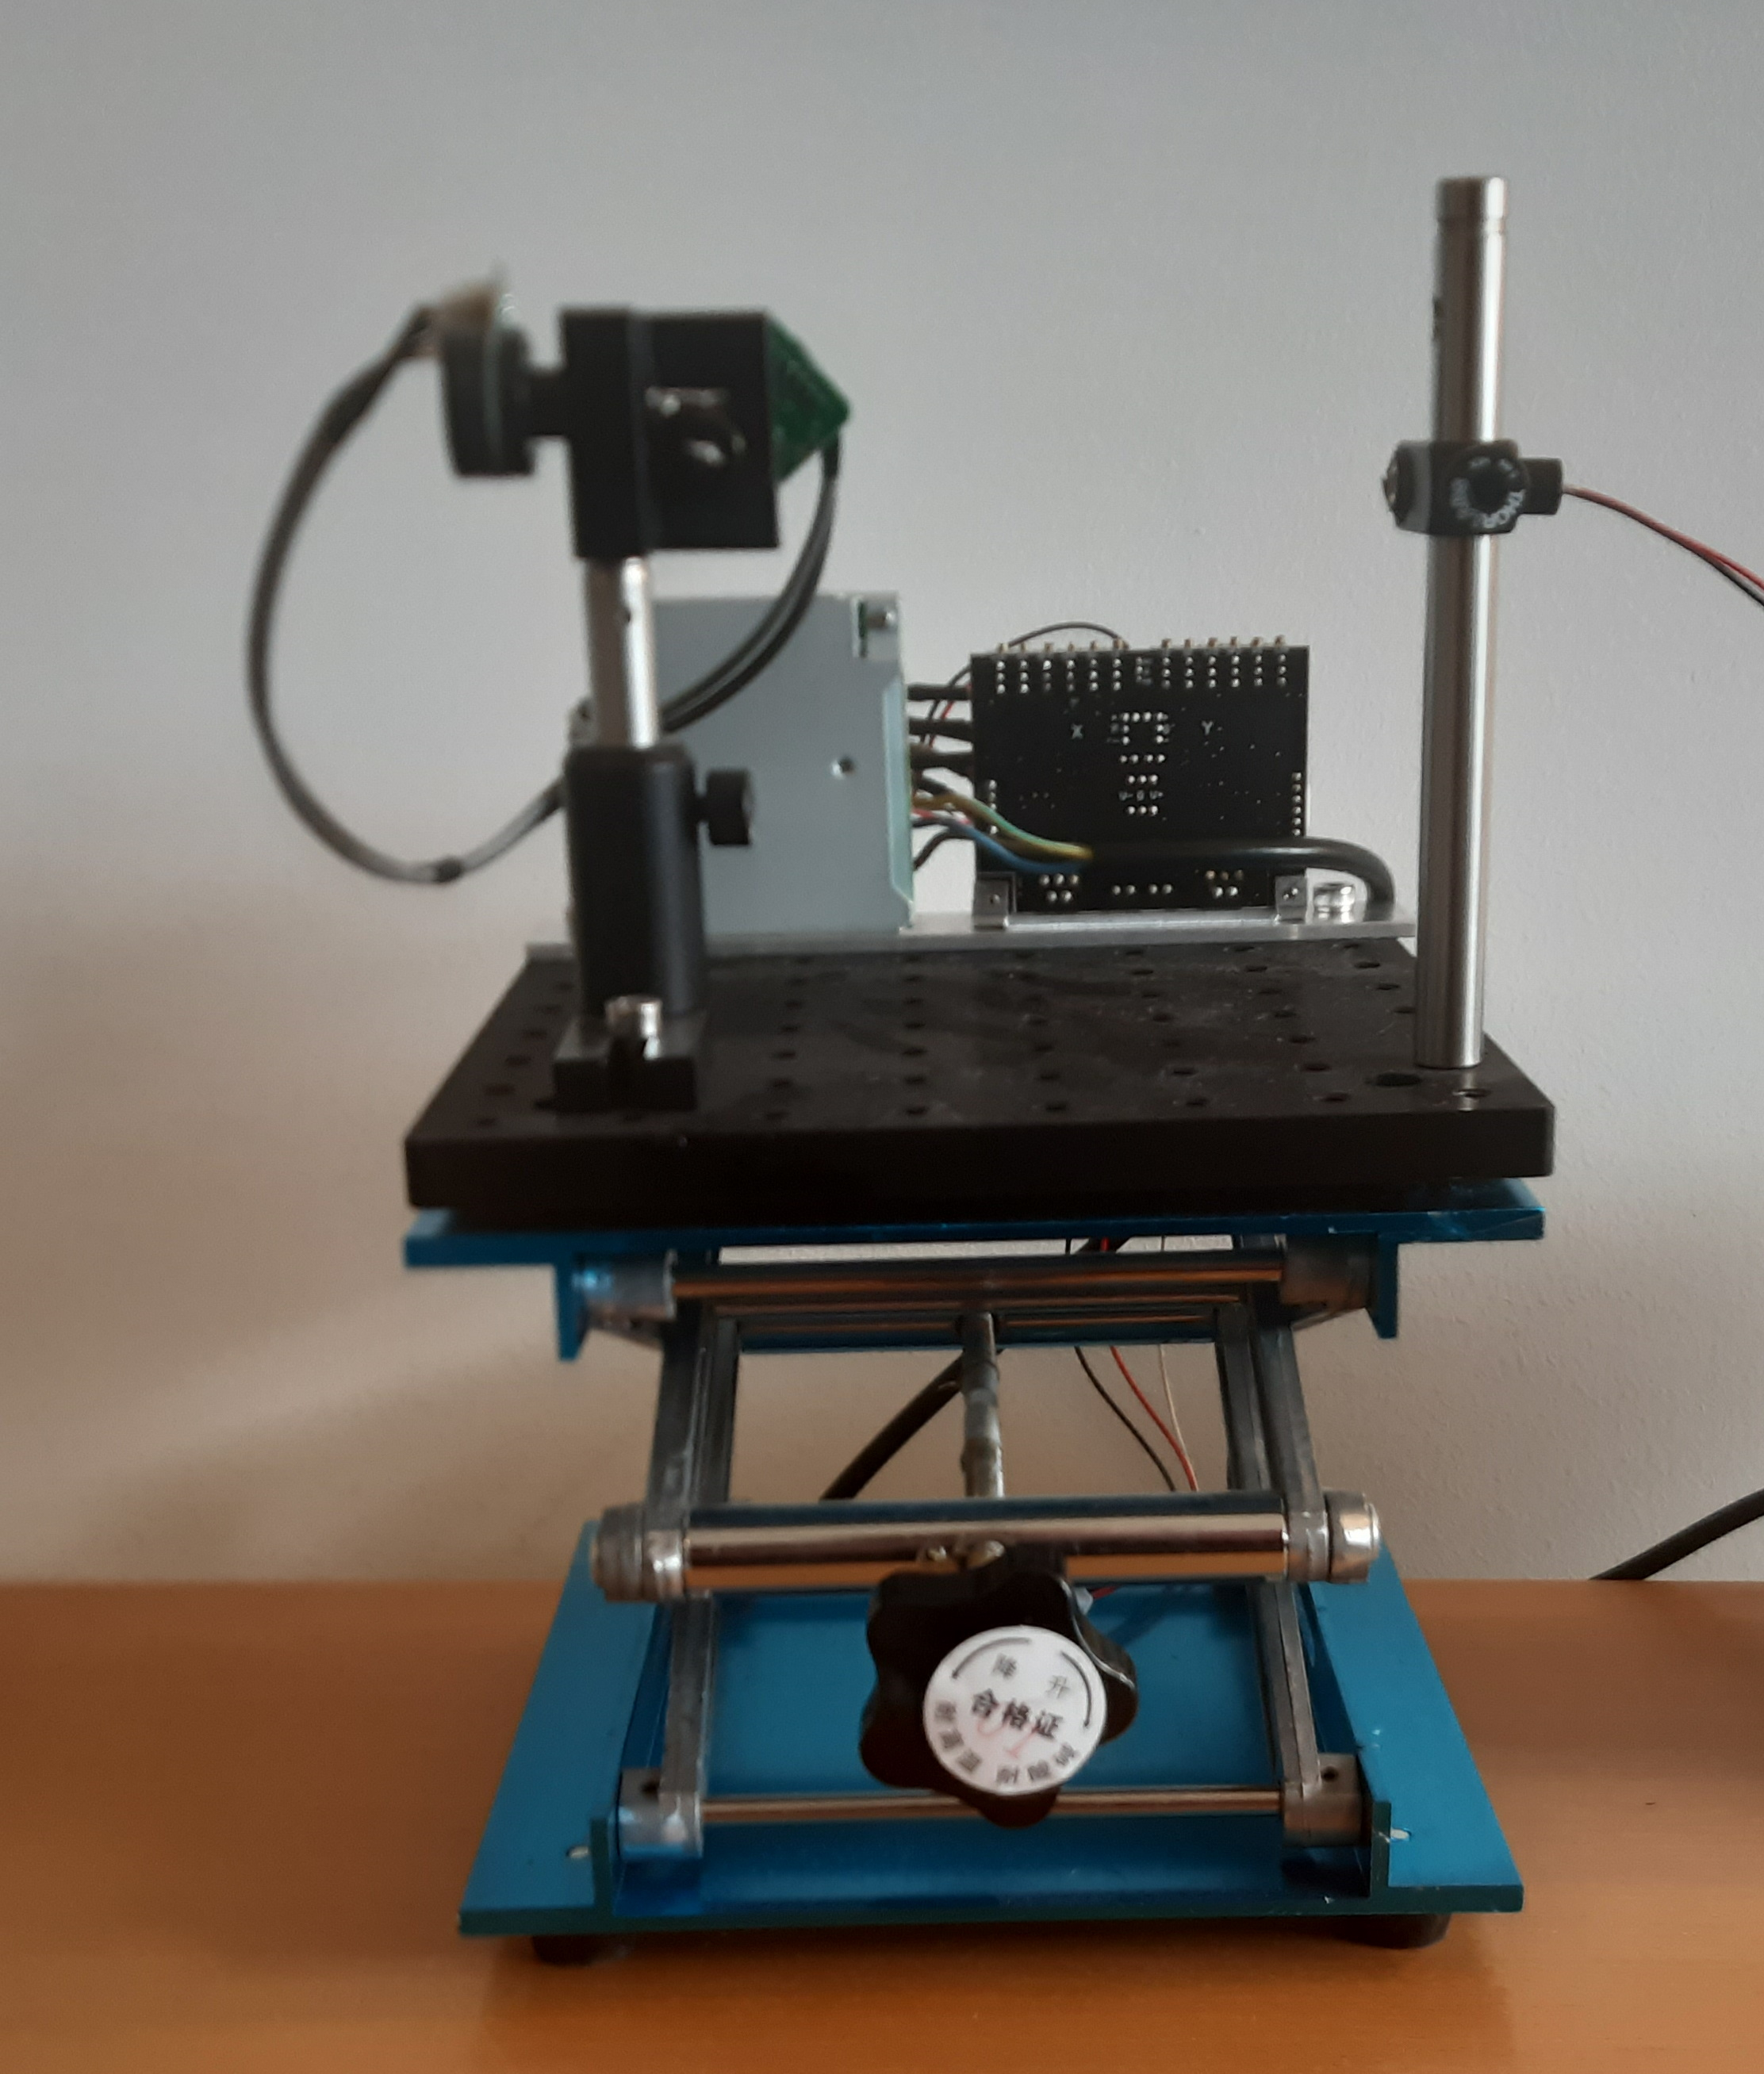
\includegraphics[width=\bildwidth]{pics/DutFront02.jpg}	\caption{DutFront02}	\label{DutFront02}	\end{figure}
% \begin{figure}[h!]	\centering	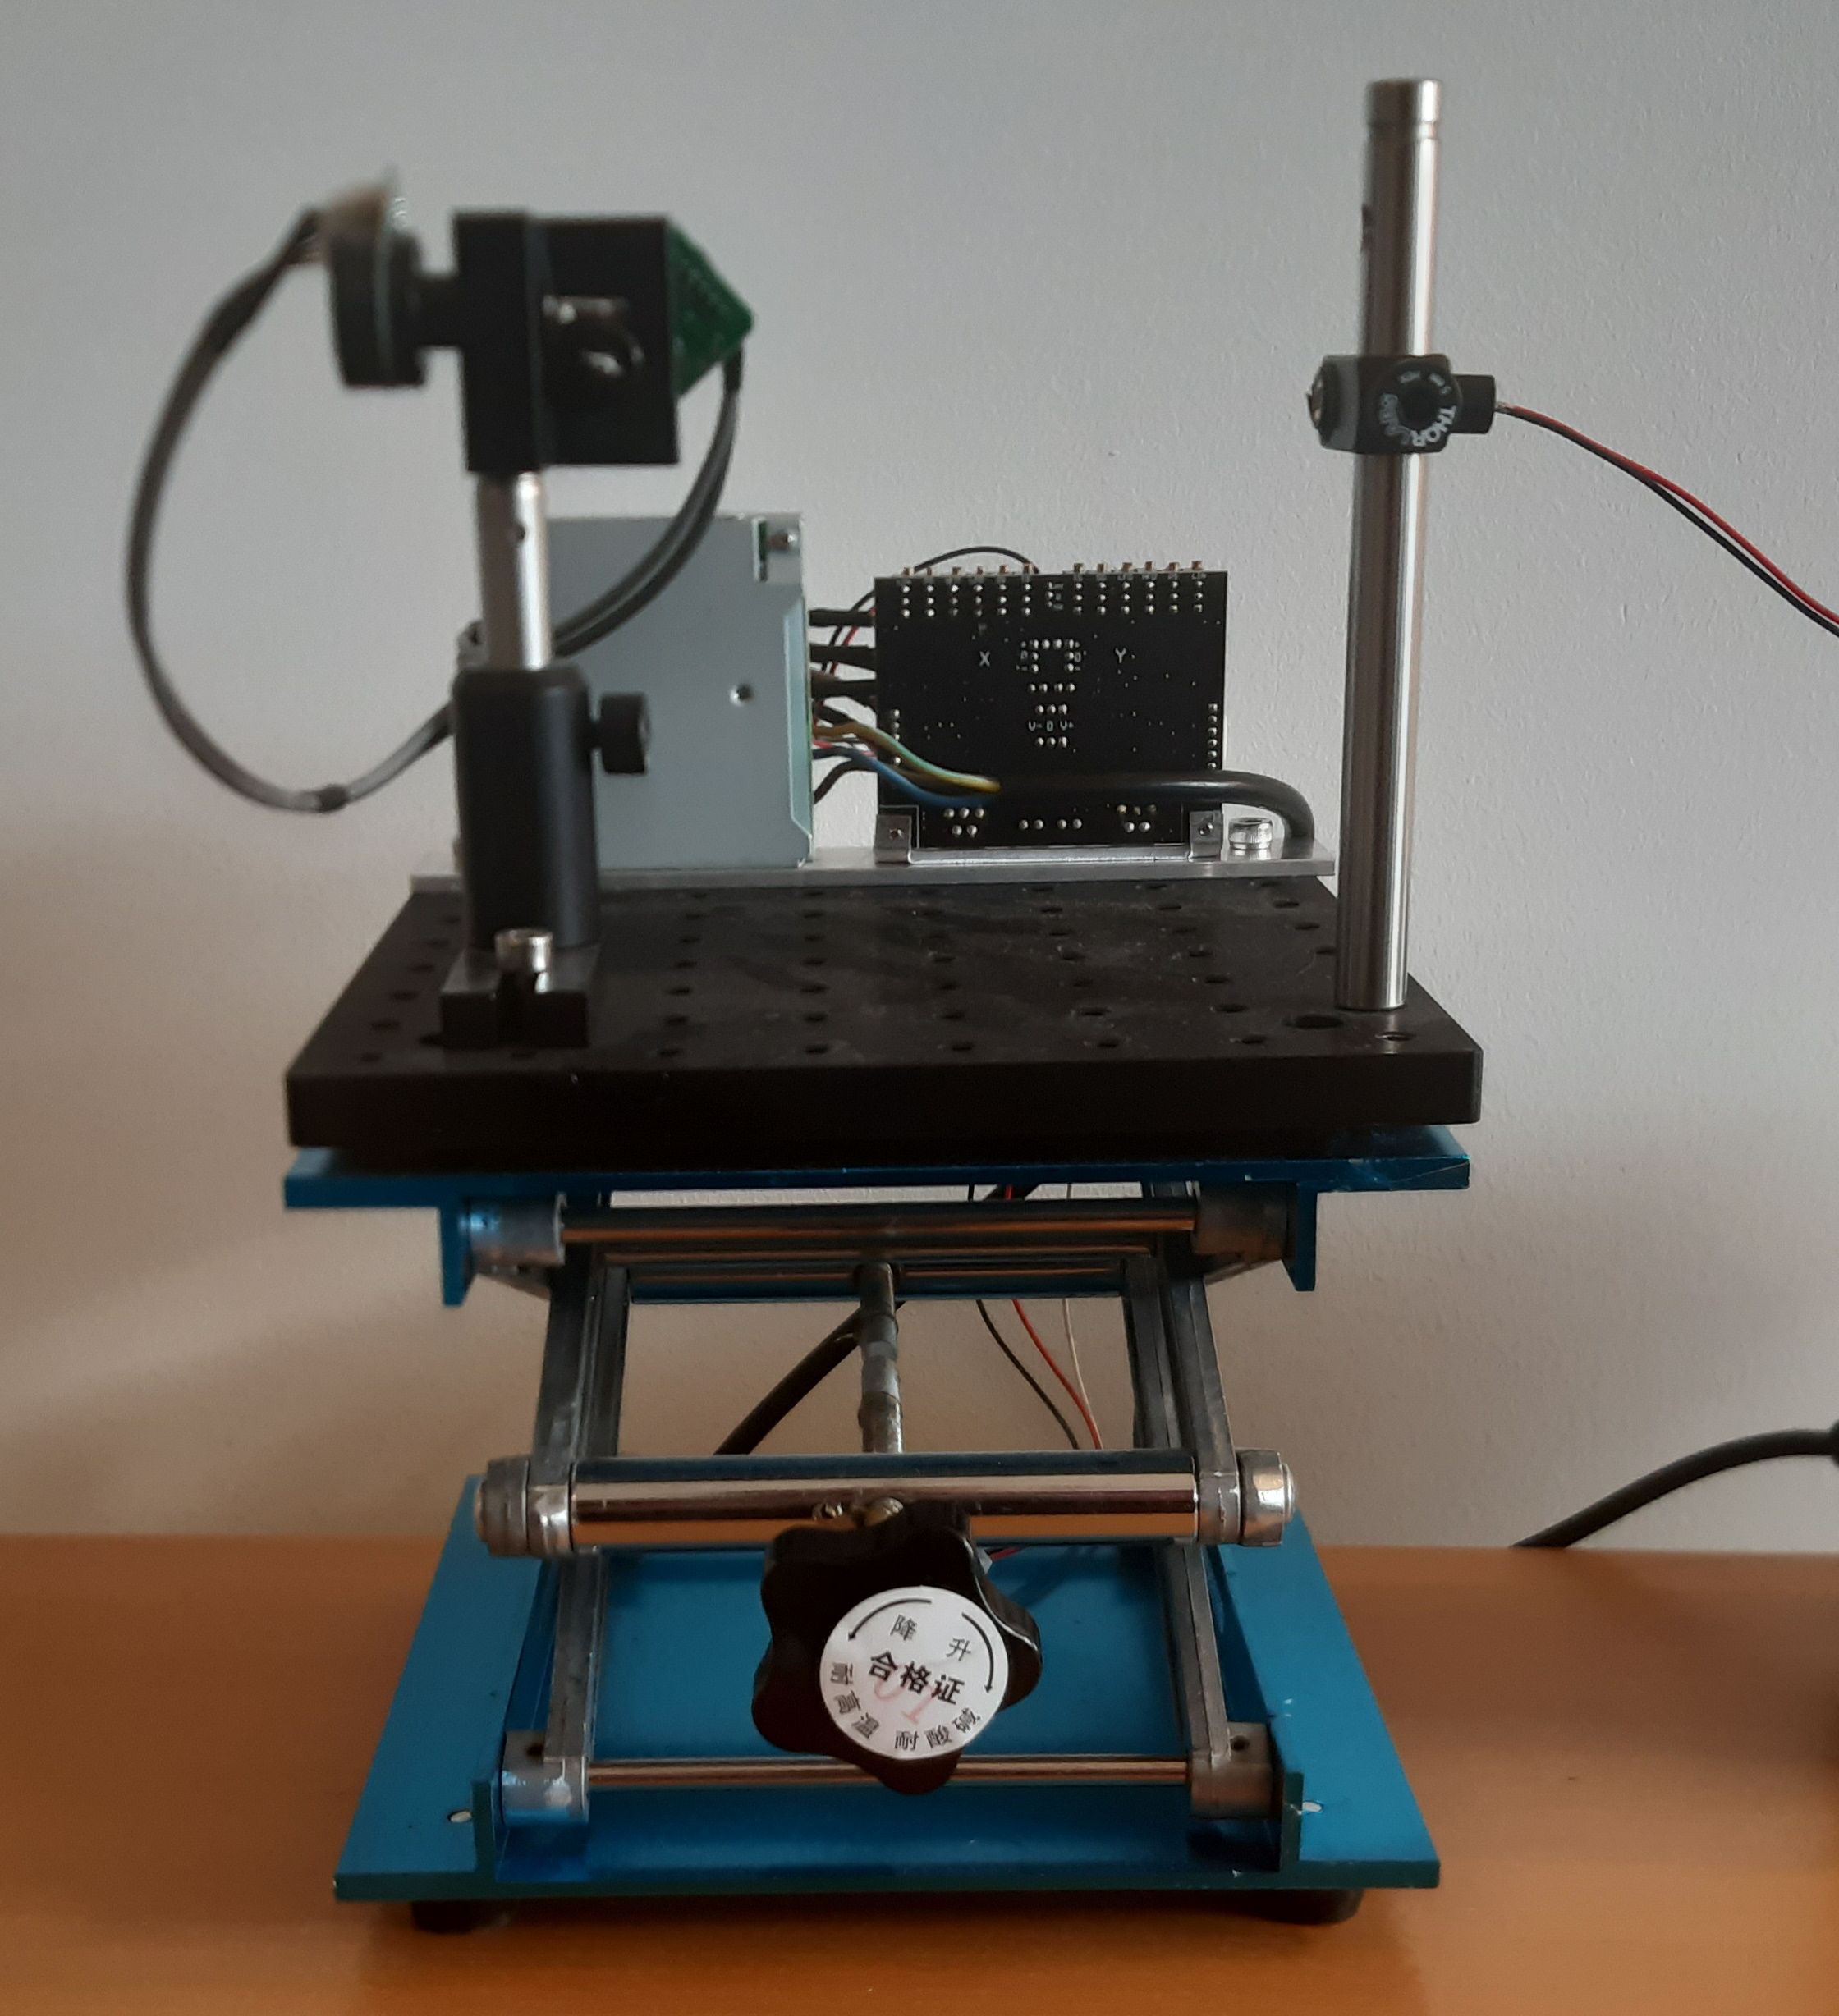
\includegraphics[width=\bildwidth]{pics/DutFront03.jpg}	\caption{DutFront03}	\label{DutFront03}	\end{figure}
% \begin{figure}[h!]	\centering	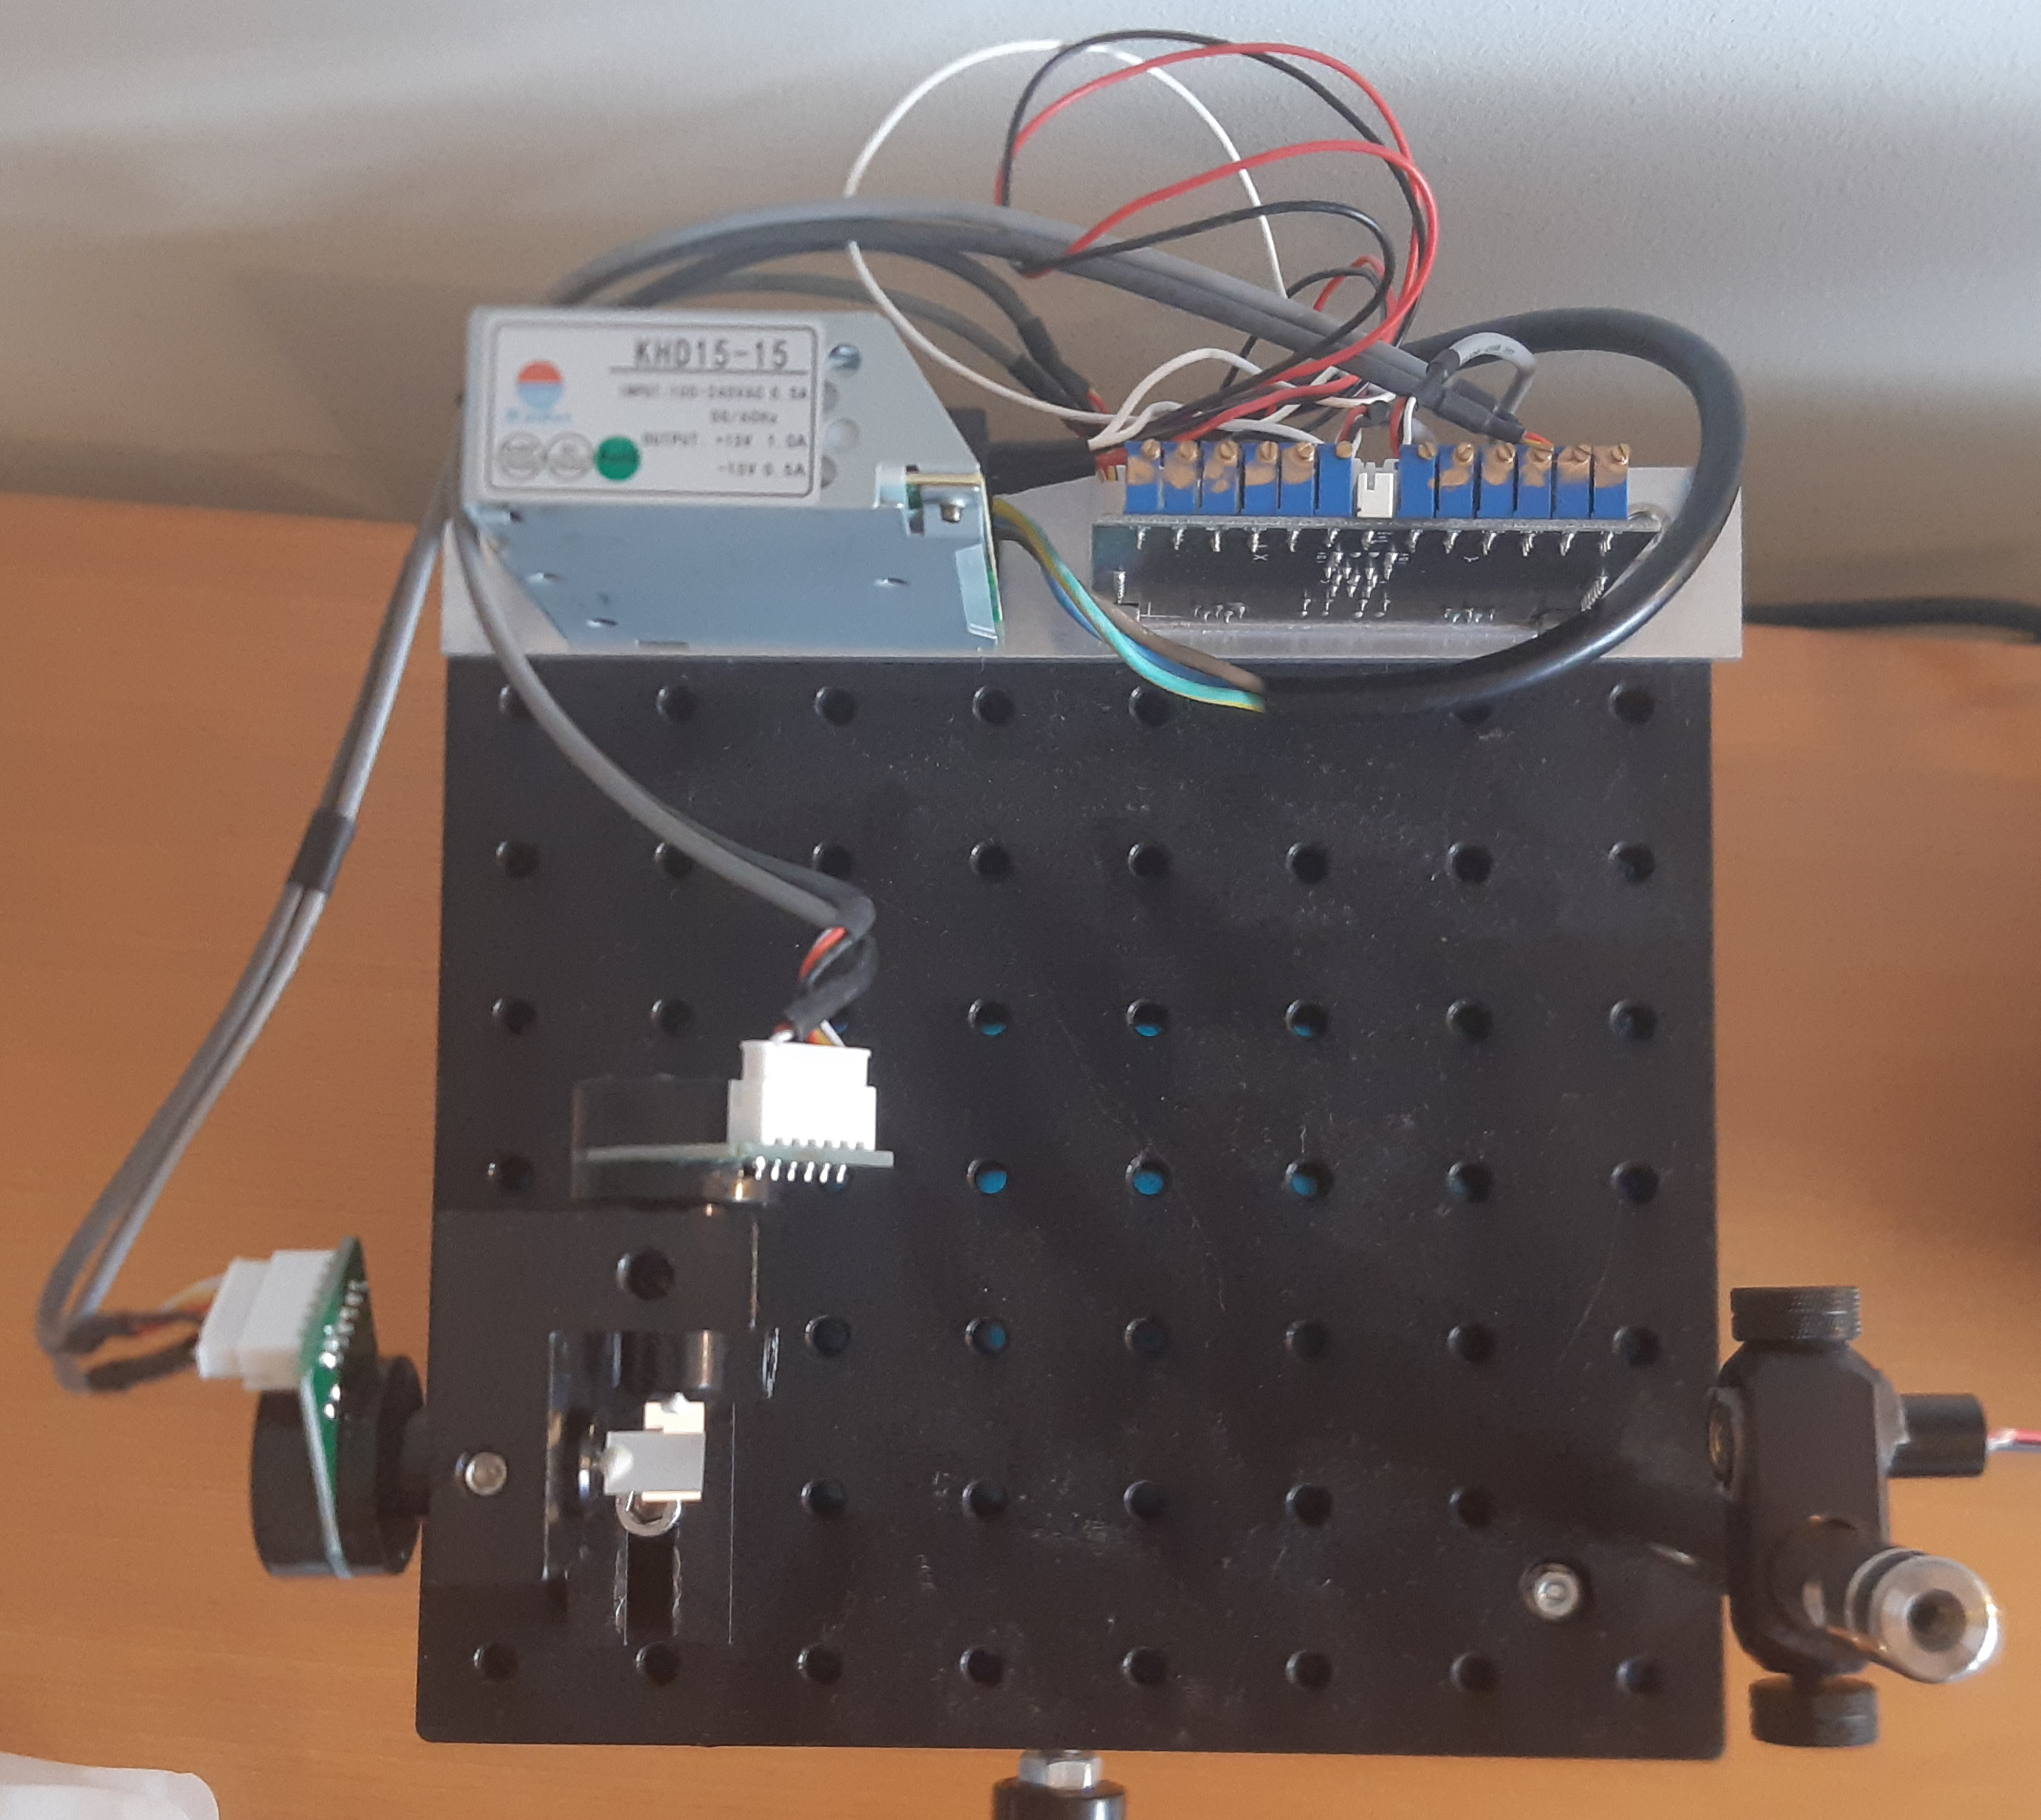
\includegraphics[width=\bildwidth]{pics/DutTop01.jpg}	\caption{DutTop01}	\label{DutTop01}	\end{figure}
\begin{figure}[h!]	\centering	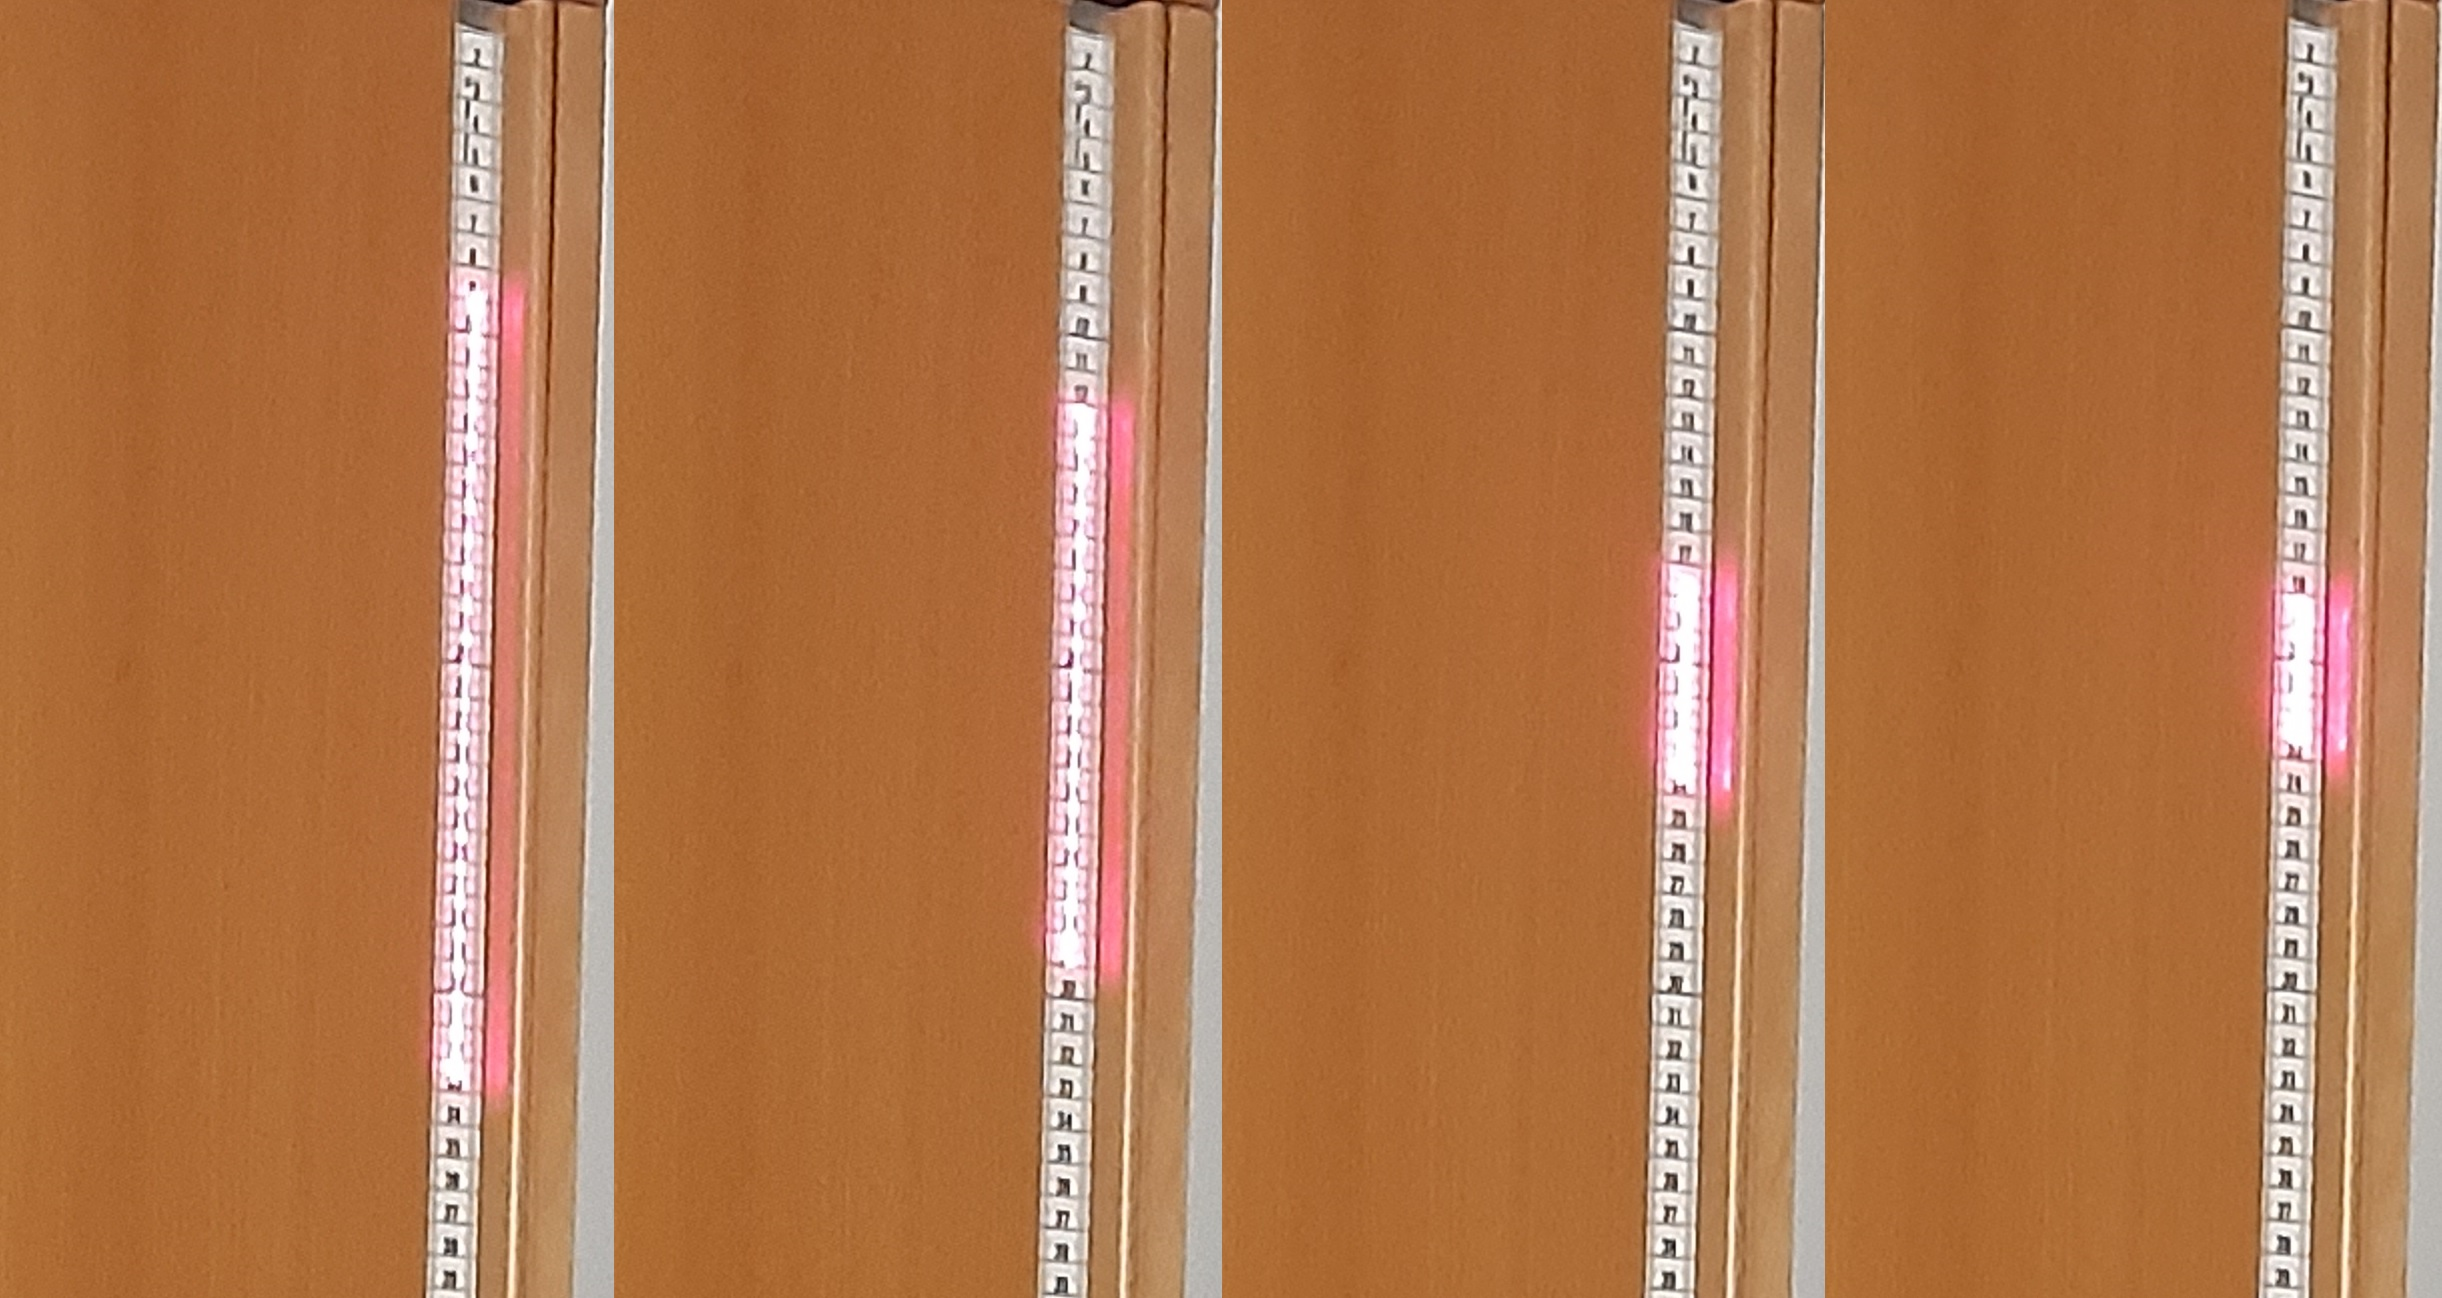
\includegraphics[width=\bildwidth]{pics/ImageMeasure01.jpg}	\caption{Abbilder von vier Messungen}	\label{ImageMeasure01}	\end{figure}
\bild{h!}{DetektorsForPhase}{Detektor zur Phasenmessung}{DetektorsForPhase}
% \begin{figure}[h!]	\centering	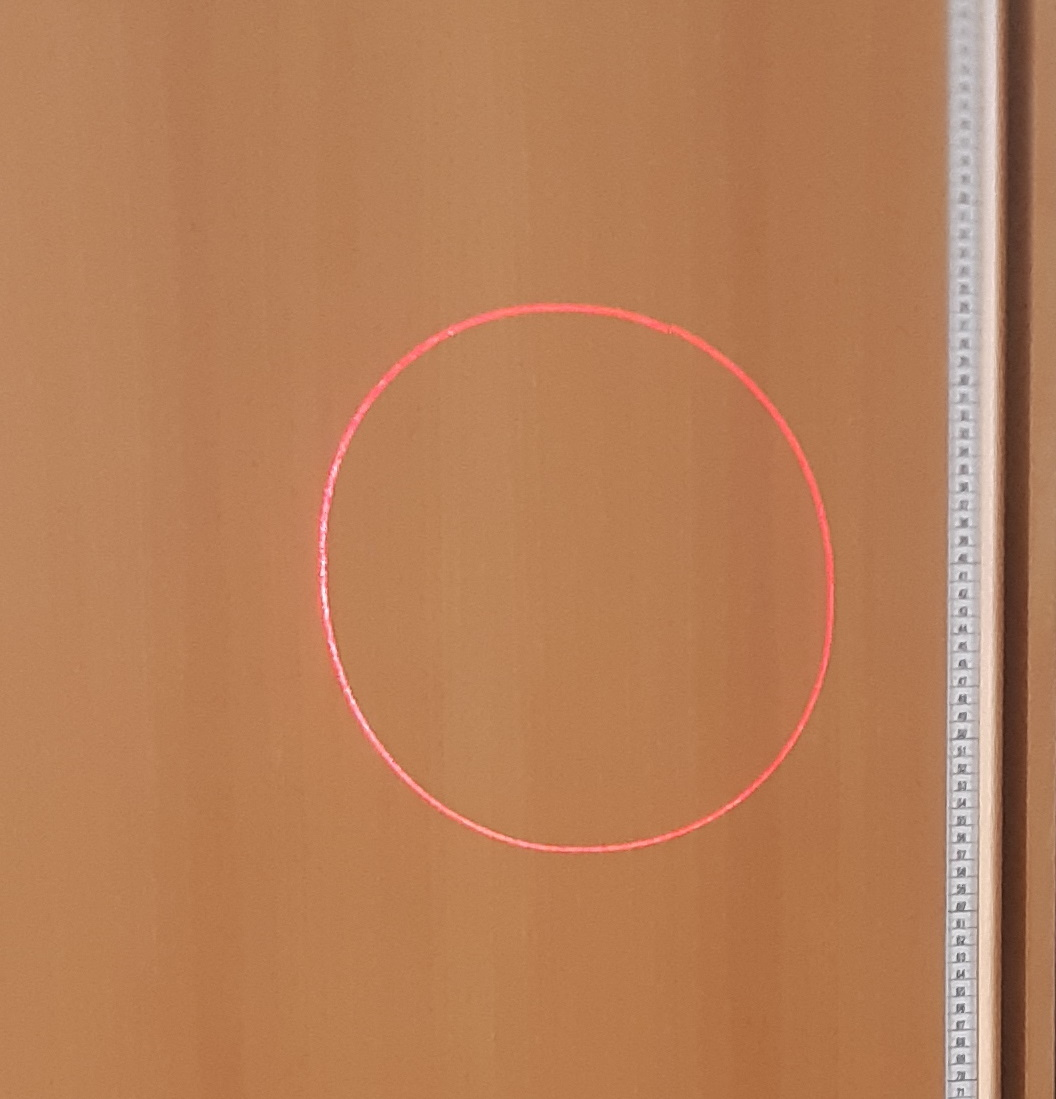
\includegraphics[width=\bildwidth]{pics/ImageXY01.jpg}	\caption{ImageXY01}	\label{ImageXY01}	\end{figure}
% \begin{figure}[h!]	\centering	\includegraphics[width=\bildwidth]{pics/.jpg}	\caption{}	\label{fig_sim}	\end{figure}

% \subsection{Messungen}
	% \begin{table}[h!]
	% \begin{center}
	% \begin{tabular}{l|l}
	% \input{Mess1.csv}
	% \end{tabular}
	% \caption{Messungcsv}
	% \label{Messungcsv}
	% \end{center}
	% \end{table}

\section{Ergebnisse}
\bild{h!}{Mess1log.eps}{Bode-Diagramm des \galvo }{Mess1log}
Die Ergebnisse der Messung sind in Abb.~\ref{Mess1log} dargestellt: Es existiert ein linearer Bereich unterhalb von 1kHz, bei dem die Auslenkung sehr exakt dem Steuersignal folgt. Oberhalb davon nimmt die Auslenkung mit steigender Frequenz ab und erreicht beim orangen Marker die -3dB-Grenzfrequenz mit 1.3kHz. Zwischen dem gruenen und roten Marker verdoppelt sich die Frequenz, was einer Oktave entspricht. Die Amplitude der Auslenkung faellt dabei um 6.43dB. Diese naeherungsweise 6dB/Oktave entsprechen 40dB/Dekade und somit einem System zweiter Ordnung der Form\cite{Staudecker}
	\begin{align*}
	% G(s) & = \frac{V}{(T_N s)^2 + 2 \xi T_N s +1} & \textrm{wird mit} \\
	% |s| & = |\alpha + j\omega| \overset{\alpha = 0} = \omega & \textrm{und} \\
	% T_N & = \frac{1}{\omega_0}  & 	\textrm{zu} \\
	G(\omega) & = \frac{V}{(\frac{\omega}{\omega_0} )^2 + 2 \xi \frac{\omega}{\omega_0}  +1} & \textrm{mit} \\
	% d &= 3190 mm \\
	\xi & = 1 \\
	\omega_0 &= 2\pi f_g \\
	f_{g}	& = 1300 Hz \\
	V &= 116.4 \frac{mm}{V} \\ % =  291mm/2.5V
	% dmax = 291mm
	% Vpp = 2.5V
	% f_{g,1Vpp} & = 1000 Hz \\
	\end{align*}
Die Daempfung $\xi$ mit '1' laesst sich aus dem Kurvenverlauf abschaetzen, da dieser keine Resonanzspitze an der Grenzfrequenz aufweist. Die Verstaerkung 'V' setzt die maximale Auslenkung mit der Amplitude der Steuerspannung ins Verhaeltnis. Auf eine Rueckrechnung von der Auslenkung auf den Drehwinkel des \galvo s wurde verzichtet. Fuer die Applikation ist die erreichbare Auslenkung in mm von Bedeutung, der Winkel stellt somit keine relevante Information dar. Beide vorhandenen  Galvanometer-Spiegel des Testobjektes wurden unter gleichen Bedingungen vermessen und zeigten nahezu identes Verhalten bezueglich ihrer Dynamik. Das Phasendiagramm ergibt sich mit der Formel \textrm{$\phi = 360^\circ f  \Delta t$} aus den gemessenen $\Delta t$. Diese wiederum stellen die Verzoegerung zwischen dem Nulldurchgang des Steuersignals, sowie der steigenden Flanke eines Opto-Detektors dar, der an der optischen Null-Position platziert ist. Der resultierende Verlauf entspricht einigermassen dem erwarteten Phasengang eines Systems 2ter Ordnung. Allerdings weist er schon bei tiefen Frequenzen eine Abweichung von der 0grad-Achse ab, was eine Totzeit des verwendeten Detektors vermuten laesst.
\section{Konklusion}
Das gewonnene Modell wird in einer Masterarbeit zur Adaptierung von Steuersignalen herangezogen. Das zugrundeliegende Konzept dazu nennt sich 'flachheitsbasierte Steuerung'. Hierbei wird das Steuersignal, unter Einbeziehung der Modell-Eigenschaften, so berechnet, dass der Ausgang einer Sollkurve folgt. Abgesehen von diesem direkten Nutzen der Messungen, verbessert sich auch das intuitive Verstaendnis der analysierten Komponenten und nuetzt damit bei der Applikation und Abschaetzung der Applizierbarkeit in OCT-Systeme. \\
Weitere Messungen mit unterschiedlichen Steuerspannungen und an mehreren Frequenzen, 	speziell im Bereich der Grenzfrequenz, sollen das bestehende Modell noch verfeinern. Auch soll die vermutete Totzeit des Opto-Detektors untersucht werden, damit praezisere Phasen-Messungen moeglich sind.

% \hfill rechtsbuendiger Text
\section*{Danksagung}
% \begin{itemize}
Martin Staudecker, Guenther Hannesschlaeger, Rankl Christian, Josef Langer und Silke Dorner, fuer die Assistenz bei Messungen.
% \end{itemize}
\label{cha:galvoChar}
